%
% The first command in your LaTeX source must be the \documentclass command.
\documentclass[sigchi]{acmart}
\usepackage{array}
\usepackage{graphicx}
\usepackage{subcaption}
\usepackage{multirow}

%
% defining the \BibTeX command - from Oren Patashnik's original BibTeX documentation.
\def\BibTeX{{\rm B\kern-.05em{\sc i\kern-.025em b}\kern-.08emT\kern-.1667em\lower.7ex\hbox{E}\kern-.125emX}}
    
% Rights management information. 
% This information is sent to you when you complete the rights form.
% These commands have SAMPLE values in them; it is your responsibility as an author to replace
% the commands and values with those provided to you when you complete the rights form.
%
% These commands are for a PROCEEDINGS abstract or paper.
\copyrightyear{2025}
\acmYear{2025}
\setcopyright{acmlicensed}
\acmConference[SNA '25]{Social Network Analysis '24}{2024/25}{University of Pisa, Italy}
\acmBooktitle{Analisi dell'affinità musicale degli artisti di Last.fm}
\acmPrice{0.00}
%\acmDOI{10.1145/1122445.1122456}
%\acmISBN{978-1-4503-9999-9/18/06}

% end of the preamble, start of the body of the document source.
\begin{document}

%
% The "title" command has an optional parameter, allowing the author to define a "short title" to be used in page headers.
\title{Analisi dell'affinità musicale degli artisti di Last.fm}

%
% The "author" command and its associated commands are used to define the authors and their affiliations.
% Of note is the shared affiliation of the first two authors, and the "authornote" and "authornotemark" commands
% used to denote shared contribution to the research.
\author{Calogero Giudice}
\email{c.giudice@studenti.unipi.it}
\affiliation{%
  \institution{Student ID: 530155}
}

\renewcommand{\shortauthors}{Calogero Giudice}


% The abstract is a short summary of the work to be presented in the article.
\begin{abstract}
Questo progetto analizza una rete di artisti musicali del social network {\itshape \href{https://www.last.fm/home}{last.fm}} in base a dei coefficienti di similarità (Sample e Jaccard Ratios) che potrebbero rappresentare delle affinità a livello stilistico o di pubblico. Sono state esaminate sia le {\bfseries caratteristiche strutturali} della rete, procedendo a svolgere una previsione, in base ai Ratios menzionati in precedenza e al coefficiente di popolarità, su possibili aumenti o cali di popolarità futuri. \\ \\ Questi risultati possono rappresentare un {\bfseries modello} che potrebbe riflettersi nello scenario musicale odierno, fornendo nuovi studi e strumenti che possono essere utili a prevedere eventuali nuovi scenari. Infatti, possono esserci artisti emergenti che potrebbero godere di maggiore popolarità futura se ben collegati, con artisti di popolarità alta e collegati con ratio alti; allo stesso tempo, si potrebbero notare alcuni artisti ritenuti popolari che potrebbero avere un trend opposto e quindi in declino.\footnote{
{\bf Project Repositories}\\
\noindent Data Collection: \url{https://github.com/Kalo9603/2024_Giudice/tree/main/data_collection}\\
\noindent Network Analysis: \url{https://github.com/Kalo9603/2024_Giudice/tree/main/network_analysis}\\
\noindent Open Problem: \url{https://github.com/Kalo9603/2024_Giudice/tree/main/open_problem}\\
\noindent Report: \url{https://github.com/Kalo9603/2024_Giudice/tree/main/report}}
\end{abstract}


%
% Keywords. The author(s) should pick words that accurately describe the work being
% presented. Separate the keywords with commas.
\keywords{Social Network Analysis, musica, {\itshape Last.fm}, affinità, similarità, popolarità}


%
% This command processes the author and affiliation and title information and builds
% the first part of the formatted document.
\maketitle

\section{Introduzione}
Nell'epoca dell'affermazione dell'industria musicale digitale, piattaforme come {\itshape \href{https://www.last.fm/home}{last.fm}} offrono tanti dati sugli artisti musicali, sulle abitudini di ascolto degli utenti e sulle relazioni tra i singoli profili musicali (gli utenti, gli artisti, gli album, etc.). Gli artisti presenti nella piattaforma sono stati analizzati sotto una prospettiva di rete sociale: si possono ipotizzare così degli scenari, dei fenomeni interessanti: la similarità tra artisti, la popolarità degli stessi, l'affermazione di artisti emergenti o l'effetto contrario. \\ \\ L'analisi parte dalla costruzione di una rete basata su coefficienti di similarità; di questi ne sono stati individuati due:

\begin{itemize}
\item Il {\itshape Sample Ratio}, ovvero l’intensità del legame tra due artisti in base ai simili condivisi.
\item Lo {\itshape Jaccard Ratio}, ovvero l’affinità relativa all’insieme totale di simili.
\end{itemize}
Matematicamente, è molto più probabile che lo {\itshape Jaccard} sia inferiore del rispettivo {\itshape Sample}, poiché il denominatore del primo è sempre maggiore del secondo (a meno che tali denominatori non coincidono). \\ \\ In parallelo si è stimata la {\bfseries popolarità} degli artisti presenti nel dataset: per far ciò ci si è basati sullo {\bfseries Z-Index}, che mette in relazione il numero di ascoltatori e quello di ascolti. Ciò ha permesso di classificare gli artisti in tre classi: {\bfseries \itshape mainstream}, {\bfseries \itshape medio} ed {\bfseries \itshape emergente}; a questi ne sono stati affiancati altri tre: {\bfseries \itshape possibile mainstream}, {\bfseries \itshape possibile medio} e {\bfseries \itshape ritorno emergente} in base al trend di (de)crescita calcolato. \\ \\ L'obiettivo principale della seconda parte del progetto è quello di identificare le caratteristiche strutturali degli artisti mainstream e di quelli emergenti ed, eventualmente, di prevedere un cambio di status in base a determinate metriche.


\section{Data Collection}

La raccolta dei dati da analizzare si è concentrata su tre fasi specifiche:
\begin{enumerate}
\item La generazione di un elenco di artisti in base agli artisti simili;
\item La creazione di una lista di archi che collegano due artisti se entrambi i coefficienti di similarità superano la soglia del $50\%$. Il {\itshape Sample Ratio} è calcolato rispetto al numero di simili condivisi, mentre lo {\itshape Jaccard Ratio} rispetto all'insieme totale dei simili;
\item Il successivo accostamento del numero di ascolti, di ascoltatori e il calcolo delle popolarità degli artisti.
\end{enumerate}
Gli elenchi degli artisti e degli artisti simili sono stati ottenuti per mezzo dell'API di {\itshape last.fm} e, tramite programmazione ad oggetti, sono state generate le altre liste. Nel complesso vi sono quattro file:

\begin{itemize}
\item {\itshape artists.csv}, una lista di 28\,870 artisti;
\item {\itshape links.csv}, un elenco di 98\,890 archi che collegano 11\,745 artisti (il 40.68\% del totale). A causa delle lunghe tempistiche è stato elaborato il dataset sul 64.26\% dei possibili archi totali (sono stati esaminati più di 267 milioni di possibili archi su oltre 416 milioni totali: $\frac{28\,870 \cdot 28\,869}{2} = 416\,724\,015$);
\item {\itshape popularity.csv}: la medesima lista di {\itshape artists.csv} con inclusi il numero di ascoltatori, quello di ascolti, il coefficiente di popolarità e il suo logaritmo;
\item {\itshape popularity\_z.csv}: la medesima lista di {\itshape popularity.csv} a cui si accoda lo Z-Index.
\end{itemize}

In particolare, i coefficienti di correlazione citati sono calcolati come segue.

\renewcommand{\arraystretch}{1.8}  % Aumenta l'altezza delle righe

\begin{table}[H]
\centering
\small
\begin{tabular}{|c|>{\centering\arraybackslash}p{4cm}|}
\hline
\textbf{Indice} & \textbf{Formula} \\
\hline
Sample Ratio &
$SR(a, b) = \frac{|S_a \cap S_b|}{k}$ \\
\hline
Jaccard Ratio &
$JR(a, b) = \frac{|S_a \cap S_b|}{|S_a \cup S_b|}$ \\
\hline
Popolarità &
$pop_i = \frac{ascolti_i}{ascoltatori_i + 1}$ \\
\hline
Popolarità logaritmica &
$pop_{\log,i} = \log(pop_i + 1)$ \\
\hline
Media &
$\mu = \frac{1}{N} \sum_{i=1}^{N} pop_{\log,i}$ \\
\hline
Deviazione standard &
$\sigma = \sqrt{\frac{1}{N} \sum_{i=1}^{N} (pop_{\log,i} - \mu)^2}$ \\
\hline
Z-Index &
$Z_i = \frac{pop_{\log,i} - \mu}{\sigma}$ \\
\hline
\end{tabular}\\[15pt]
\caption{Formule utilizzate per la classificazione e l'analisi strutturale}
\end{table}


\subsection{Dati selezionati}

Al fine di avere un dataset iniziale di artisti si è pensato, partendo da quattro artisti provenienti da quattro generi musicali diversi (\href{https://www.last.fm/music/Annalisa}{Annalisa} per il pop italiano; \href{https://www.last.fm/music/Giorgio+Vanni}{Giorgio Vanni} per le sigle, \href{https://www.last.fm/music/Katy+Perry}{Katy Perry} per la quota internazionale e \href{https://www.last.fm/music/Ado}{Ado} per il mercato giapponese). \\ \\ Quindi, partendo da essi, viene creata la lista di artisti simili a cominciare da quelli di partenza: se non è presente, l'artista trovato viene aggiunto in lista. La medesima operazione viene svolta, alla prima iterazione, sui primi quattro artisti; poi, dalla seconda, si considerano anche tutti quelli aggiunti in coda. In questo modo è stato ottenuto un dataset di 28\,870 artisti. Relativamente all'ordine di inserimento nel dataset, a ciascun artista è stato assegnato un ID autoincrementale. \\ \\ Al termine si è passati, basandosi sull'elenco degli artisti, alla generazione del dataset dei {\itshape links} del grafo. Per far ciò per ciascun artista della lista, sfruttando le proprietà di un grafo non orientato:

\begin{itemize}
\item Si considera l'artista con ID immediatamente successivo;
\item Per la coppia in esame si prendono i rispettivi insiemi di artisti simili e si calcolano i ratio, le cui formule sono specificate nel formulario precedente;
\item Se entrambi il Sample e lo Jaccard Ratio raggiungono la soglia del 50\%, l'arco viene registrato nel dataset;
\item Si prosegue il calcolo con l'artista successivo con il medesimo algoritmo fino a raggiungere la fine della lista degli artisti.
\end{itemize}
In questo modo, ad esempio, il primo nodo (Annalisa) farà 28\,869 iterazioni, il secondo (Giorgio Vanni) 28\,868, e così via. Quindi gli ultimi nodi faranno molte meno iterazioni rispetto ai primi perché le altre possibili coppie vengono esaminate dai nodi precedenti. \\ \\ Per migliorare ulteriormente la velocità del processo è stato adottato il {\itshape multiprocessing}, in modo che più processi lavorino in parallelo sullo stesso set di artisti. Dati i tempi relativamente lunghi del processo, l'analisi del dataset è iniziato non appena il numero di artisti all'interno dei dataset dei {\itshape links} ha raggiunto la soglia richiesta. Al termine sono stati collegati 11\,745 artisti con 98\,890 archi.


\section{Network Characterization}

Si esamina qui di seguito il grafo ottenuto dalla fase di Data Collection. \\ \\ Come anticipato in precedenza, partendo da 28\,870 artisti è stato ottenuto un grafo, analizzando il 64,26\% dei possibili archi, formato da 11\,745 artisti a 98\,890 archi. \\ \\ La densità quindi è molto bassa, ovvero di $ 1.433 \times 10^{-3}$; questo è dovuto principalmente al fatto di aver adottato una soglia minima di Jaccard Ratio più alta. Infatti, matematicamente, la probabilità che lo Jaccard Ratio di un arco abbia valore minore del rispettivo Sample è nettamente maggiore, in quanto il denominatore del rapporto (vedasi la tabella nel paragrafo precedente) risulta maggiore di un valore fisso come nel Sample. \\ \\ Riassumendo, le prime generalità del grafo sono le seguenti:

\begin{table}[H]
\centering
\small
\begin{tabular}{|c|>{\raggedright\arraybackslash}p{4cm}|}
\hline
\textbf{Artisti totali} &
$ 28\,870 $ \\
\hline
\textbf{Artisti nel grafo} &
$ 11\,745 $ (40,68\%)  \\
\hline
\textbf{Archi} &
$ 98\,890 $ \\
\hline
\textbf{Densità} &
$ 1.433 \times 10^{-3} $ \\
\hline
\end{tabular}\\[15pt]
\caption{Prime generalità del grafo}
\end{table}

\subsection{Distribuzione di grado}

Il grado medio del grafo è di $ 8.42 $. \\ Per calcolarlo sono stati utilizzati, per completezza, due metodi:

\begin{itemize}
\item Dividendo il numero di righe del dataset per il numero di artisti connessi;
\item Dividendo la somma dei gradi dei singoli artisti per il numero degli stessi.
\end{itemize}
Nota che l'errore tra i due metodi è dell'ordine di $ 10^{-4} $. Dal grafico si evince la forte asimmetria del grado medio degli artisti: ve ne sono molti con grado basso e meno con grado più alto.

\begin{figure}[H]
\centering
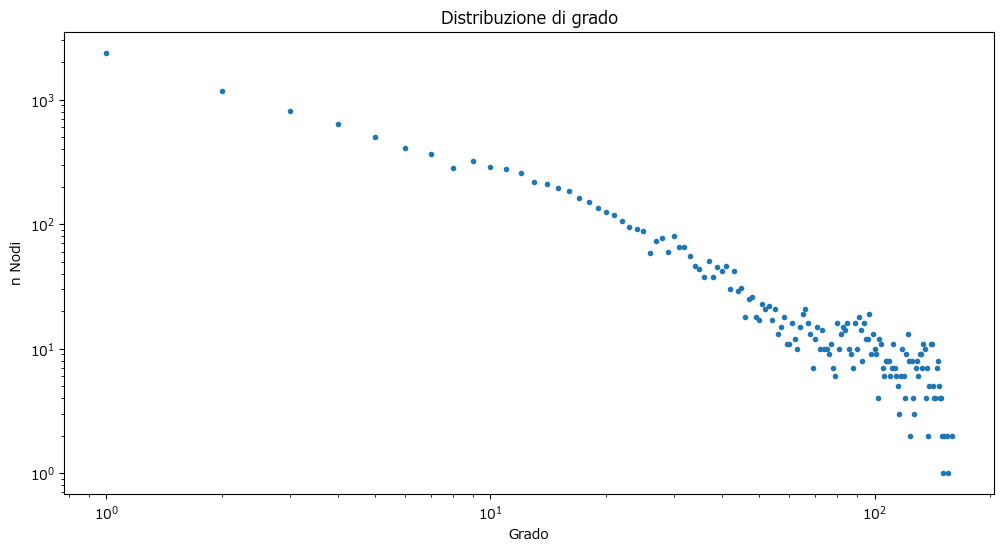
\includegraphics[width=0.45
\textwidth]{../network_analysis/plots/2_2/grDist.png}
\caption{Distribuzione del grado degli artisti}
\label{fig:grDist}
\end{figure}

\noindent Questa asimmetria dei gradi del grafo si mostra maggiormente dalle distribuzioni CDF e CCDF: la probabilità di trovare un artista con grado elevato decresce.

\begin{figure}[H]
\centering
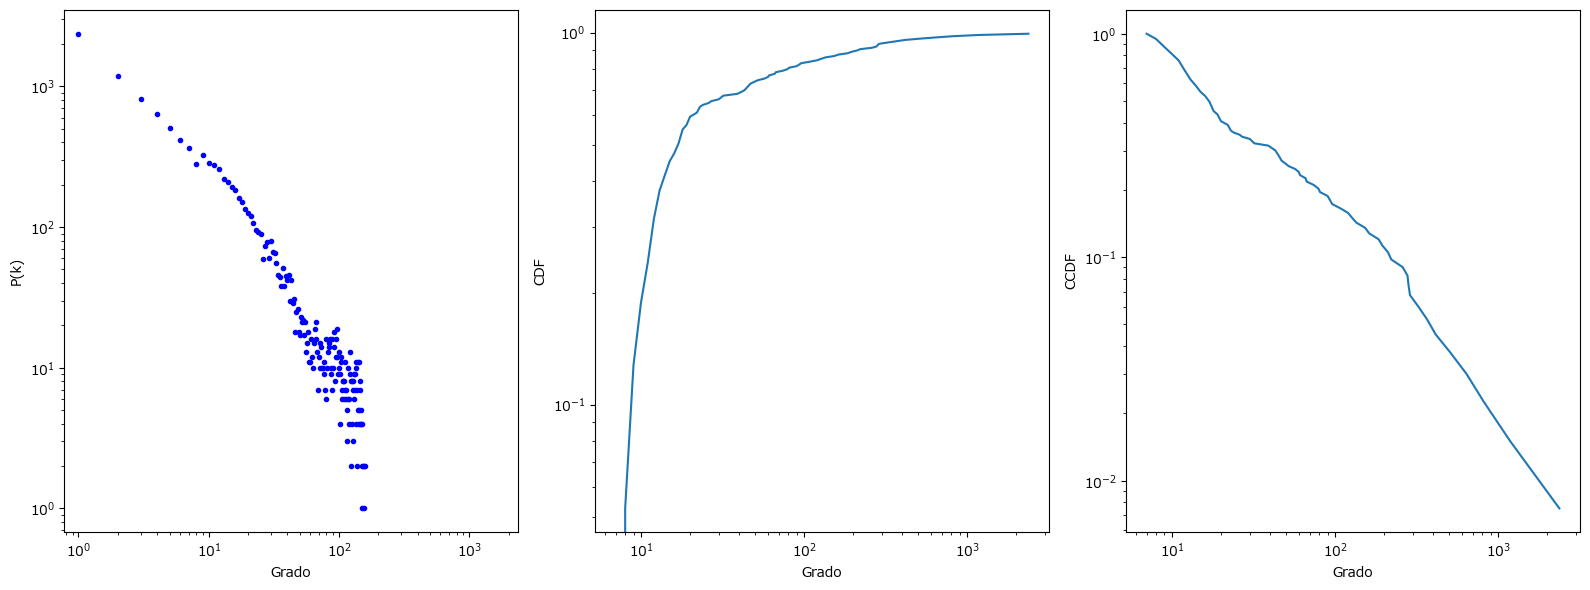
\includegraphics[width=0.45
\textwidth]{../network_analysis/plots/2_2/plotDist.png}
\caption{Distribuzione del grado degli artisti - CDF e CCDF}
\label{fig:plotDist}
\end{figure}

\noindent Dato che si tratta di un grafo pesato su due livelli, è interessante mostrare come si comportano i rispettivi pesi. Per cui si illustrano i medesimi grafici ma pesati: qui è evidente come lo Jaccard Ratio risulta più traslato indietro rispetto al Sample corrispondente. dai grafici CDF e CCDF si nota come il range dei gradi pesati Jaccard sia molto più variabile rispetto al Sample. Risulta altresì interessante la continua sovrapposizione di entrambi i gradi nel modello CCDF:

\begin{figure}[H]
\centering
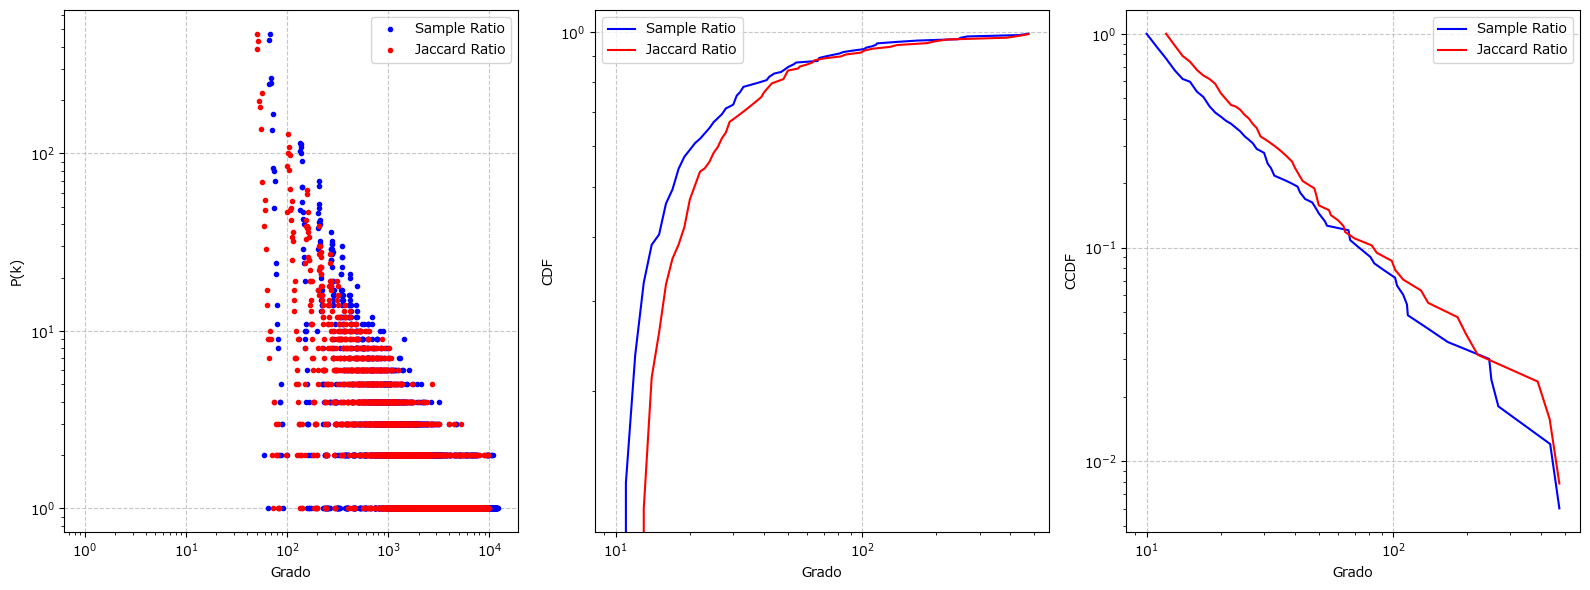
\includegraphics[width=0.45
\textwidth]{../network_analysis/plots/2_2/wPlotDist.png}
\caption{Distribuzione del grado pesato degli artisti - CDF e CCDF}
\label{fig:wPlotDist}
\end{figure}

\subsection{Confronto con il grafo ER}

Il grafo è stato confrontato con un corrispettivo Erdős-Rényi (ER) con lo stesso numero di archi e la stessa densità. Come da definizione, la distribuzione è simil-parabolica e i valori, data la densità relativamente bassa, poco appaiati.

\begin{figure}[H]
\centering
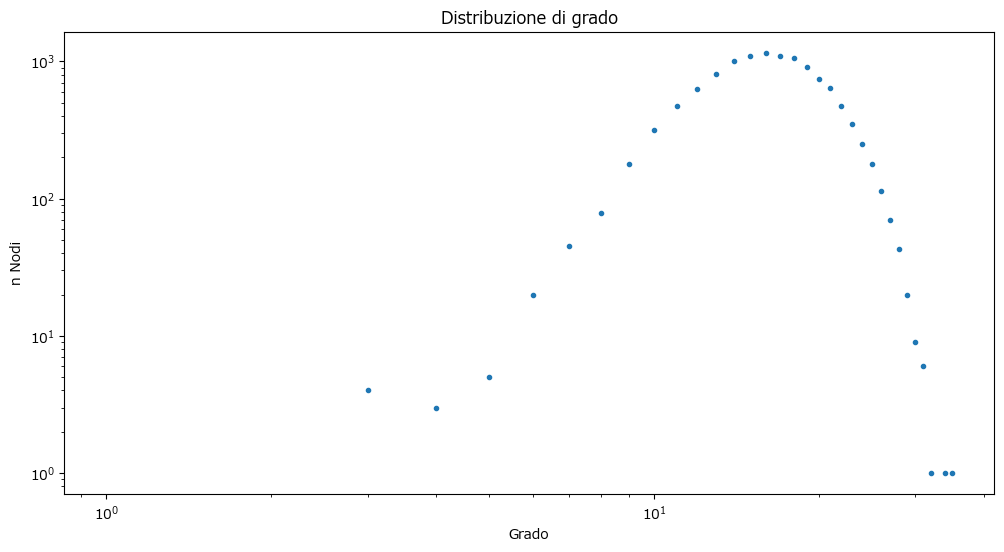
\includegraphics[width=0.45
\textwidth]{../network_analysis/plots/2_2/ERGrDist.png}
\caption{Grafo ER corrispondente}
\label{fig:ERGrDist}
\end{figure}


\subsection{Confronto con il grafo BA}

In maniera speculare è stato creato anche un corrispettivo Barabási-Albert (BA), formato da un unico componente, con lo stesso numero di archi e come parametro $m$, si è scelto il valore di default ($m=3$); la sua densità è minore del grafo principale e ha più di un terzo degli archi. Il regime è {\itshape Supercritical}.

\begin{figure}[H]
\centering
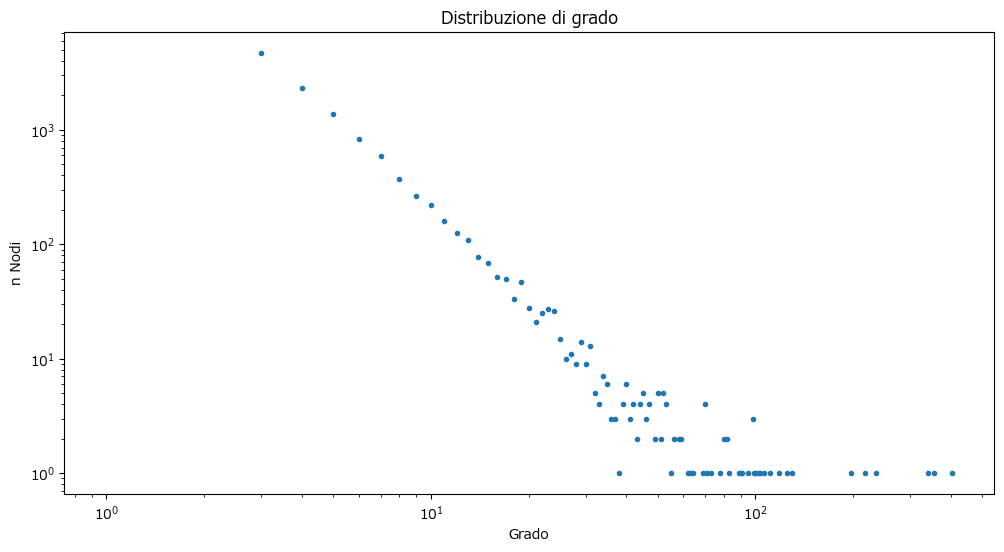
\includegraphics[width=0.45
\textwidth]{../network_analysis/plots/2_2/BAGrDist.png}
\caption{Grafo BA corrispondente}
\label{fig:BAGrDist}
\end{figure}

\noindent Dunque sono state messe a confronto le tre distribuzioni: per grado $n\approx10$ tutti e tre tendono a coincidere. Le generalità dei tre grafi sono le seguenti:

\begin{table}[H]
\centering
\renewcommand{\arraystretch}{1.3}
\resizebox{0.45\textwidth}{!}{
\begin{tabular}{|l|c|c|c|}
\hline
& \textbf{Originale} & \textbf{ER} & \textbf{BA} \\
\hline
Nodi & \multicolumn{3}{|c|}{11\,745}  \\
\hline
Archi & 98\,890 & 98\,479 & 35\,226 \\
\hline
Densità & $1.433 \times 10^{-3}$ & $1.427 \times 10^{-3}$ & $5.107 \times 10^{-4}$ \\
\hline
Clustering medio & 0.516 & $1.46 \times 10^{-3}$ & $5.163 \times 10^{-3}$ \\
\hline
Grado medio & 8.42 & 16.77 & 6 \\
\hline
Regime & \multicolumn{2}{|c|}{{\itshape Connected}} & {\itshape Supercritical} \\
\hline
\end{tabular}
}
\caption{Confronto tra le metriche del grafo e dei modelli ER e BA}
\label{tab:comparison}
\end{table}

\noindent La tabella sopra è accompagnata dal grafico sovrapposto seguente che mostra come la distribuzione del grafo si avvicini a quello BA:

\begin{figure}[H]
\centering
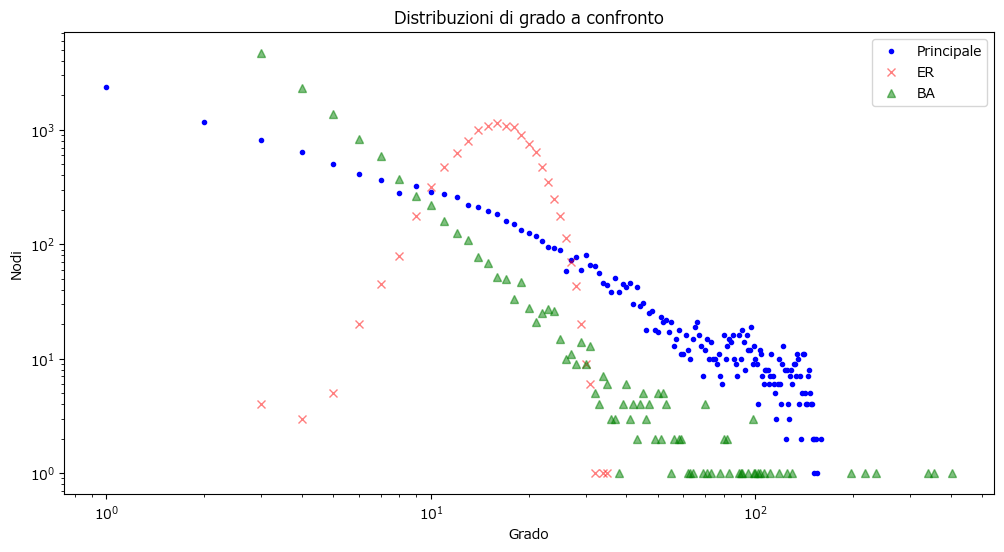
\includegraphics[width=0.45
\textwidth]{../network_analysis/plots/2_2/grComparison.png}
\caption{Confronto tra le tre distribuzioni}
\label{fig:grComparison}
\end{figure}

\noindent Si può constatare che il grafo, per quanto possa somigliare a un grafo BA, non si può prendere perfettamente a modello, complici il numero di archi e la densità nettamente minori del BA rispetto all'originale. Invece a occhio, se si sovrapponesse la medesima distribuzione pesata, si può notare che essa risulti molto più simile al BA rispetto al corrispettivo {\itshape unweighted}. Invece l'ER, sebbene alcuni valori di riferimento sono abbastanza vicini, non si approssima minimamente alla distribuzione in analisi.

\subsection{Distribuzione dei Ratio}

Stabilito il criterio per la creazione degli archi si è pensato di svolgere una breve analisi anche sulla distribuzione normale dei ratio del dataset. Mettendo in relazione il ratio con la rispettiva frequenza, si possono mettere a confronto le gaussiane. Tenendo conto che si sta visualizzando nell'intervallo $[50,100]$, la curva del Sample Ratio si mostra più "alta" e più "centrata", mentre quella dello Jaccard più bassa, omogenea, ma più dislocata a sinistra. Questo anche perché, appunto, lo Jaccard medio ($57.39\%$) risulta nettamente inferiore del corrispettivo Sample medio ($72.69\%$).

\begin{figure}[H]
\centering
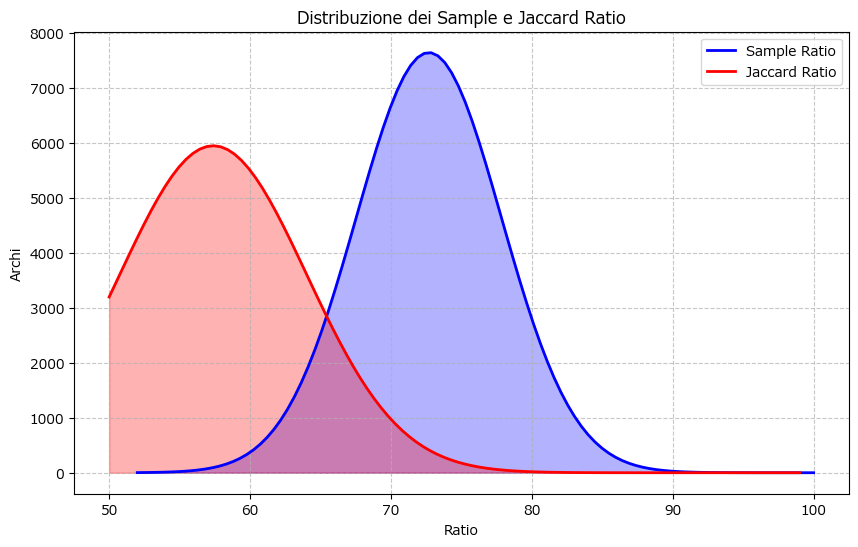
\includegraphics[width=0.45
\textwidth]{../network_analysis/plots/2_3/rtDist.png}
\caption{Distribuzione dei Sample e Jaccard Ratio}
\label{fig:rtDist}
\end{figure}

\subsection{Componenti connesse}

A causa delle soglie stabilite è stato previsto che il grafo in analisi sia molto frammentato: con l'analisi svolta sono state individuate $800$ componenti connesse. Il componente maggiormente connesso è formato da ben $920$ nodi: esso è formato da musicisti britannici o, più in generale, di molti artisti degli anni Settanta e Ottanta. Il sottografo menzionato, sia con gli archi Sample Ratio che con quelli Jaccard Ratio, è il seguente:

\begin{figure}[H]
\centering
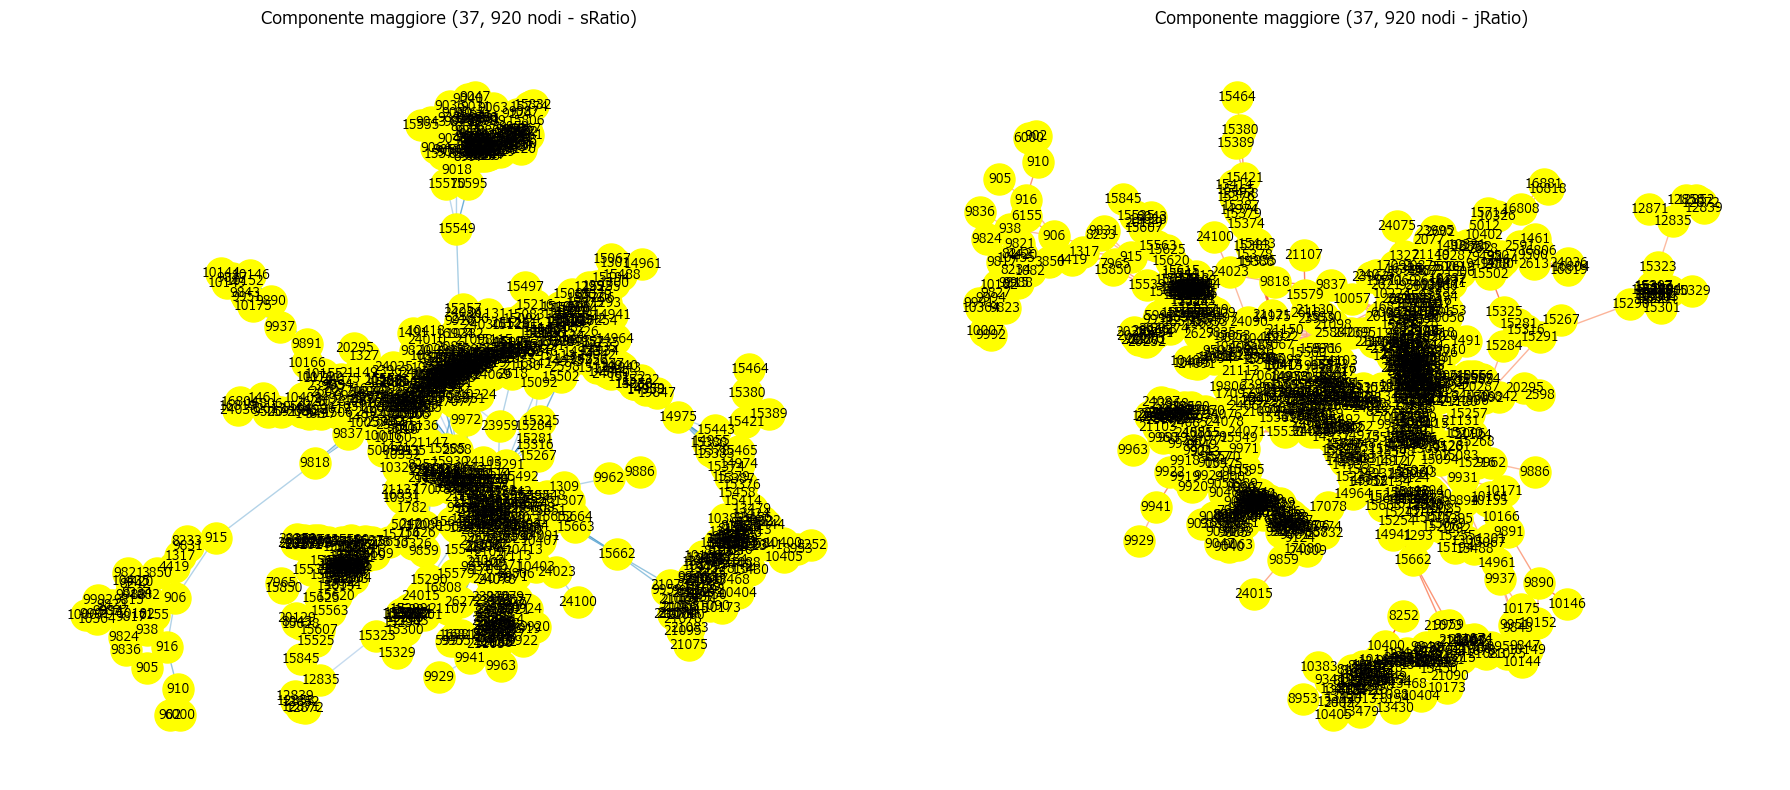
\includegraphics[width=0.45
\textwidth]{../network_analysis/plots/2_4/lrgstCmpnt.png}
\caption{Sottocomponente maggiore}
\label{fig:lrgstCmpnt}
\end{figure}

\subsection{Path Analysis}

Il numero dei sottografi è molto alto, per cui si è pensato di studiare come ne sono distribuiti i diametri. Dalla figura sotto si evince che più della metà dei sottografi sono formati da al più due nodi connessi da un singolo arco e, di conseguenza, ci sono pochi, pochissimi sottografi di diametro elevato. Il diametro medio è poco più che $2$: quindi, in media, i sottografi sono formati maggiormente da $3$-$4$ nodi:

\begin{figure}[H]
\centering
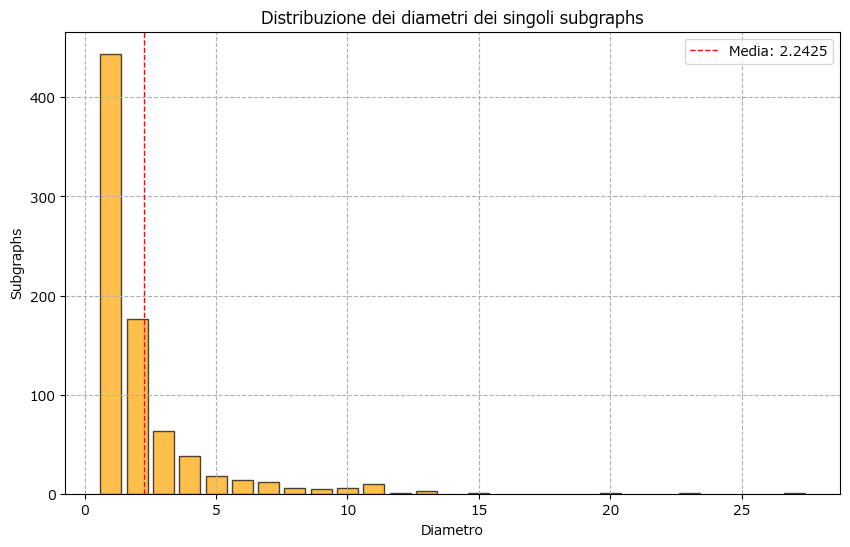
\includegraphics[width=0.45
\textwidth]{../network_analysis/plots/2_5/dmtDist.png}
\caption{Distribuzione dei diametri dei subgraphs}
\label{fig:dmtDist}
\end{figure}

\subsection{Clustering e Densità}

Il clustering medio è di $0.51646$. In media, quindi, più vi sono poco più della metà di vicini collegati tra di loro, per ciascun nodo. Questo valore suggerisce che nella rete ci sono tante triadi o, comunque, gruppi piccoli di artisti; per cui gli artisti simili tendono a connettersi tra di loro in maniera abbastanza moderata. \\ \\ Parallelamente a ciò, come è stato specificato in tabella, si è esaminato come sono distribuite le densità dei sottografi. In maniera speculare al grafico precedente, tutti i sottografi con diametro $1$ hanno densità massima. Al contrario, maggiore è il diametro del sottografo, minore è la probabilità di avere una densità alta: per questi motivi la densità media per sottografo è decisamente più alta rispetto a quella globale ($0.7713$ per sottografi, $1.433 \times 10^{-3}$ globale)

\begin{figure}[H]
\centering
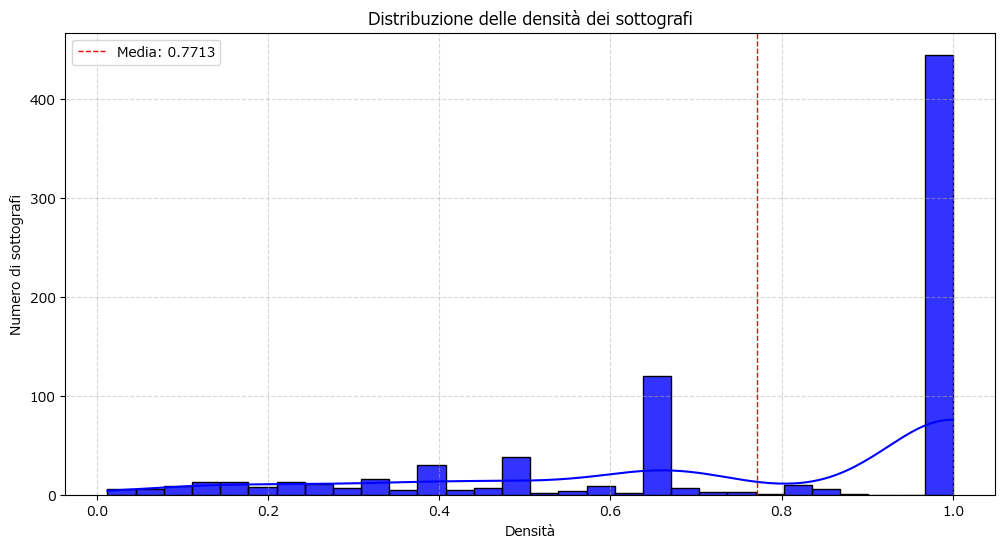
\includegraphics[width=0.45
\textwidth]{../network_analysis/plots/2_6/densDist.png}
\caption{Distribuzione delle densità dei subgraphs}
\label{fig:densDist}
\end{figure}


\subsection{Centralities}

Sono state esaminate sia la {\itshape Closeness} che la {\itshape Betweenness} Centrality. Su questi parametri salta all'occhio che i valori massimi sono entrambi molto bassi, il che suggerisce una certa lontananza (in termini di Closeness) o di dominanza (per la Betweenness). Queste sono conseguenze nell'aver stabilito una soglia minima di Ratio relativamente centrale: infatti, la probabilità che due artisti siano legati da un ratio basso è ben maggiore. \\ \\ I valori massimi di {\bfseries Closeness} Centrality oscillano tra $1.347 \times 10^{-2}$ e $1.429 \times 10^{-2}$: ciò suggerisce che, sebbene la soglia è relativamente bassa risulta coerente in quanto la rete è poco densa. La top $20$ degli artisti per Closeness è dominata da artisti provenienti dal mondo country e country pop; inoltre può anche suggerire che all'interno del dataset gli artisti country sono collegati in maniera migliore rispetto agli altri generi musicali. Si mostra un grafico che mostra i $20$ artisti con maggiore Closeness:

\begin{figure}[H]
\centering
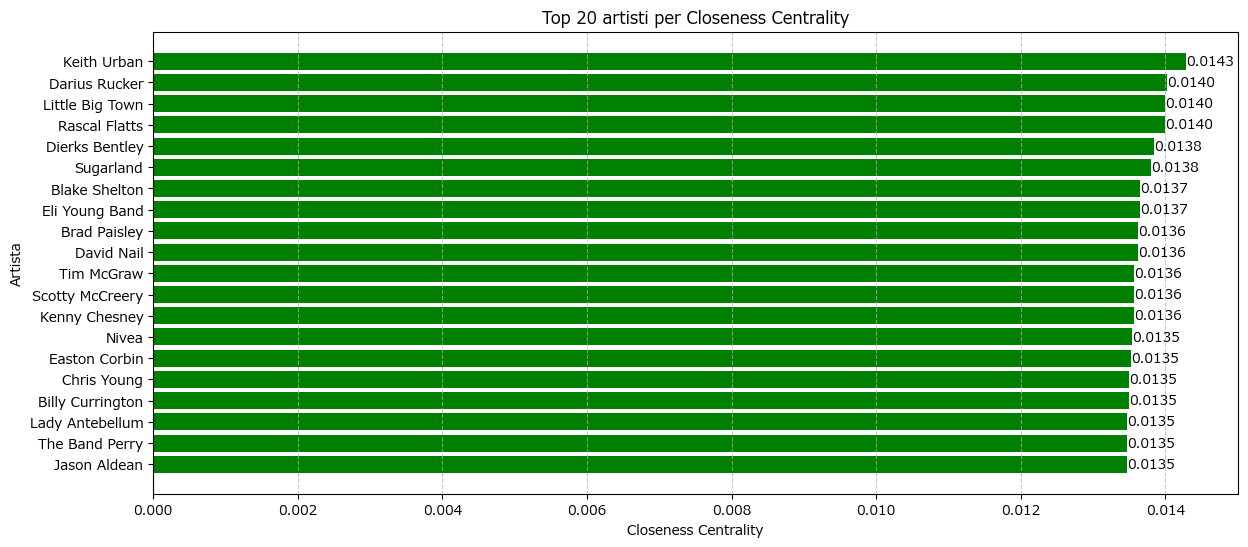
\includegraphics[width=0.45
\textwidth]{../network_analysis/plots/2_7/top20Clness.png}
\caption{I primi 20 artisti per Closeness Centrality}
\label{fig:top20Clness}
\end{figure}

\noindent I primi $20$ valori di {\bfseries Betweenness}, invece, si trovano in un range tra $8.6 \times 10^{-4}$ e $2.95 \times 10^{-3}$: valori così bassi implicano una non dipendenza di artisti per mantenere la rete connessa, sia perché è formata da molte componenti connesse, sia perché il numero di archi è esiguo. \\ \\ Può anche suggerire una struttura abbastanza distribuita e quindi vi sono molti percorsi alternativi. Si nota che gli artisti con maggiore Betweenneess sono meno mainstream e più eterogenei. Vi sono, infatti, artisti rock degli anni Ottanta, Classic Rock e artisti giapponesi, tra i quali di Alternative Rock/Metal; essi non sono al centro del grafo, ma fungono da ponti tra comunità diverse.

\begin{figure}[H]
\centering
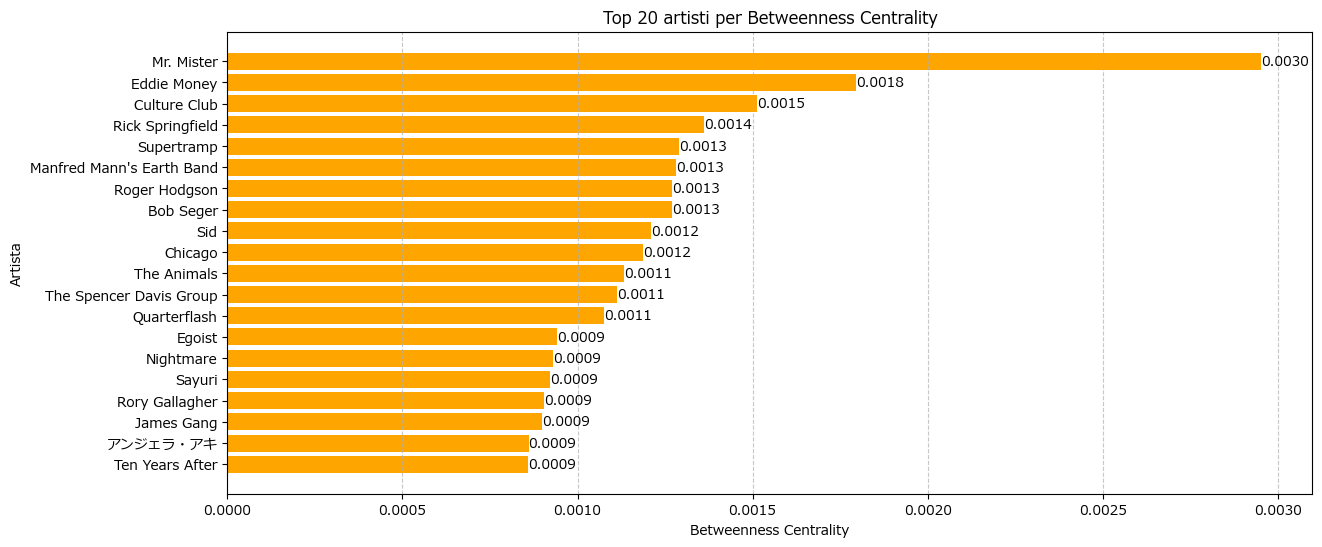
\includegraphics[width=0.45
\textwidth]{../network_analysis/plots/2_7/top20Btwnss.png}
\caption{I primi 20 artisti per Betweenness Centrality}
\label{fig:top20Btwnss}
\end{figure}

\section{Task: Open Question}

Come {\itshape Open Question} si è pensato di indagare su come è possibile distinguere gli artisti mainstream da quelli emergenti, in termini di centralità, densità e distribuzione delle connessioni. Inoltre si prova a prevedere se, in base ai Ratio e alla popolarità, un artista può avere la possibilità di diventare più conosciuto o, se le condizioni sono sfavorevoli, tornare poco conosciuto.

\subsection{Generalità e definizione dei parametri}

L'indagine comincia con il calcolo della {\itshape popolarità} di un artista. Come già specificato nella Table 1, la popolarità è stata calcolata come il rapporto tra il numero di ascolti e il numero di ascoltatori aumentato di $1$ (in modo da non avere problemi di calcolo). \\ \\ Per uniformare i {\itshape gap}, cioè per non avere popolarità troppo distanti l'una dall'altra e quindi per non agevolare molto gli artisti con pochi ascoltatori e molti ascolti, si è optato di utilizzare il suo logaritmo e, al fine di un riferimento con la media $\mu$ e la deviazione standard $\sigma$ della popolarità, è stato calcolato lo Z-Index. Il valore è direttamente proporzionale alla distanza dalla media; il segno, invece, indica se l'artista si trova sopra/sotto la media stessa. Dalla Table 1 si riprendono le formule relative alla popolarità:

\begin{table}[H]
\centering
\small
\begin{tabular}{|c|>{\centering\arraybackslash}p{4cm}|}
\hline
\textbf{Indice} & \textbf{Formula} \\
\hline
Popolarità &
$pop_i = \frac{ascolti_i}{ascoltatori_i + 1}$ \\
\hline
Popolarità logaritmica &
$pop_{\log,i} = \log(pop_i + 1)$ \\
\hline
Media &
$\mu = \frac{1}{N} \sum_{i=1}^{N} pop_{\log,i}$ \\
\hline
Deviazione standard &
$\sigma = \sqrt{\frac{1}{N} \sum_{i=1}^{N} (pop_{\log,i} - \mu)^2}$ \\
\hline
Z-Index &
$Z_i = \frac{pop_{\log,i} - \mu}{\sigma}$ \\
\hline
\end{tabular}\\[15pt]
\caption{Formule utilizzate per la classificazione}
\end{table}

\noindent Dai calcoli si evince che la popolarità logaritmica media, cioè il valore in cui lo Z-Index è nullo, è uguale a $2.768$. I valori uscillano da $0$ (quattro coppie di artisti senza ascolti, né ascoltatori) a $6.62$ (Lyodra); questo vuol dire che la scala è abbastanza omogenea.

\subsection{Definizione delle classi}

Per poter definire se un artista è emergente, mainstream o sulla via di mezzo, sono stati adottati i quantili. Se un artista ha uno Z-Index:

\begin{itemize}
\item minore o uguale al $15^\circ$ percentile, allora è considerato {\itshape emergente};
\item maggiore o uguale all\textquotesingle$85^\circ$ percentile, allora è considerato {\itshape mainstream};
\item in tutti gli altri casi è {\itshape medio}.
\end{itemize}
Il seguente grafico mostra la dsitribuzione dello Z-Index con evidenziati i quantili di riferimento:

\begin{figure}[H]
\centering
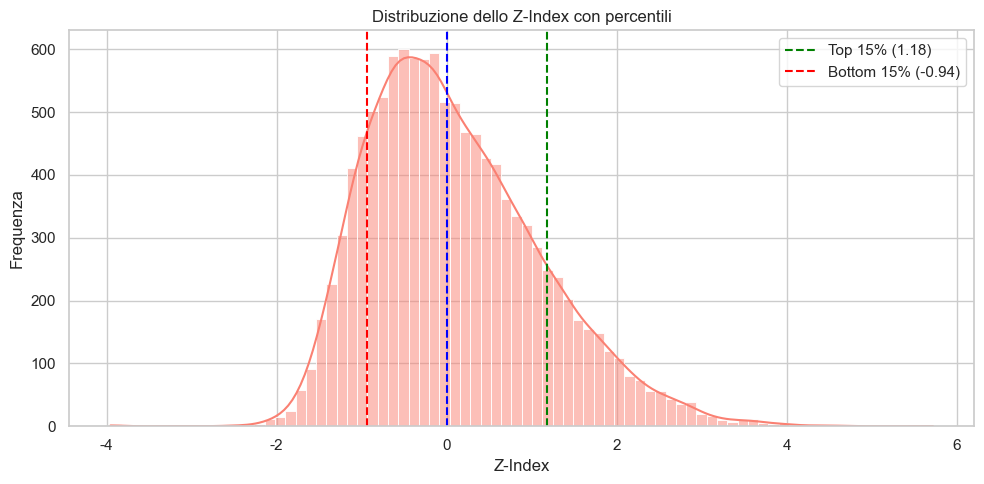
\includegraphics[width=0.45
\textwidth]{../open_problem/plots/3_2/popDistPc.png}
\caption{Distribuzione dello Z-Index con quantili}
\label{fig:popDistPc}
\end{figure}

\noindent Gli artisti considerati emergenti si trovano al più {\itshape a sinistra} della retta in rosso, i mainstream al più {\itshape a destra} della retta in verde, infine i medi in mezzo le due rette citate. \\ \\ Considerati questi parametri si è provato ad accostare tali classi agli archi del grafo: in questo modo si otterranno delle coppie del tipo {\itshape mainstream}-{\itshape mainstream}, {\itshape mainstream}-{\itshape medio}, ecc. Da ciò è stata creata una {\itshape heat map} che mostra come sono accoppiate le classi di artisti tra di loro:

\begin{figure}[H]
\centering
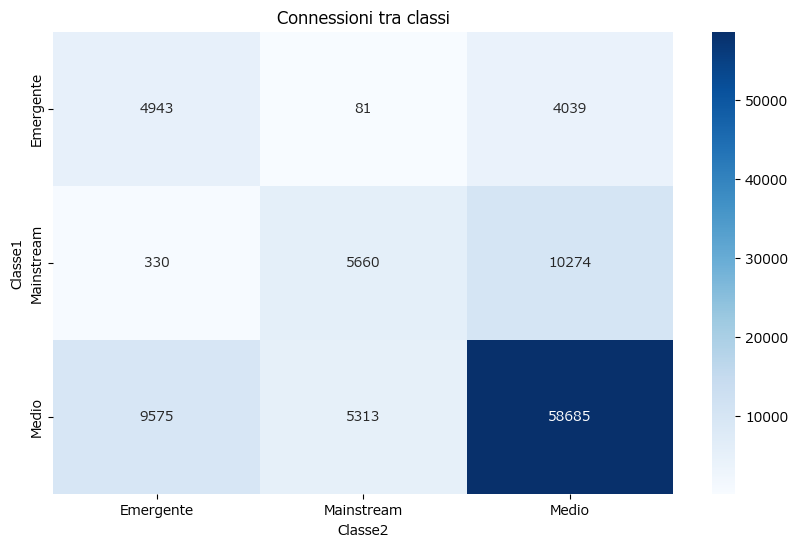
\includegraphics[width=0.45
\textwidth]{../open_problem/plots/3_2/clConnection.png}
\caption{Connessioni tra le classi}
\label{fig:clConnection}
\end{figure}

\noindent Un dato interessante che salta all'occhio è che gli archi tra artisti mainstream ed emergenti è decisamente più basso degli altri ($330+81=411$ su 98\,890, solo lo $0.41\%$ del totale). Per cui è molto meno probabile che un emergente possa saltare direttamente al mainstream; dunque l'artista in questione dovrà necessariamente passare dalla classe intermedia. \\ \\ Andando più nel dettaglio si è creato un {\itshape box plot} che mostra come sono distribuiti i Ratio in base alle classi sopra:

\begin{figure}[H]
\centering
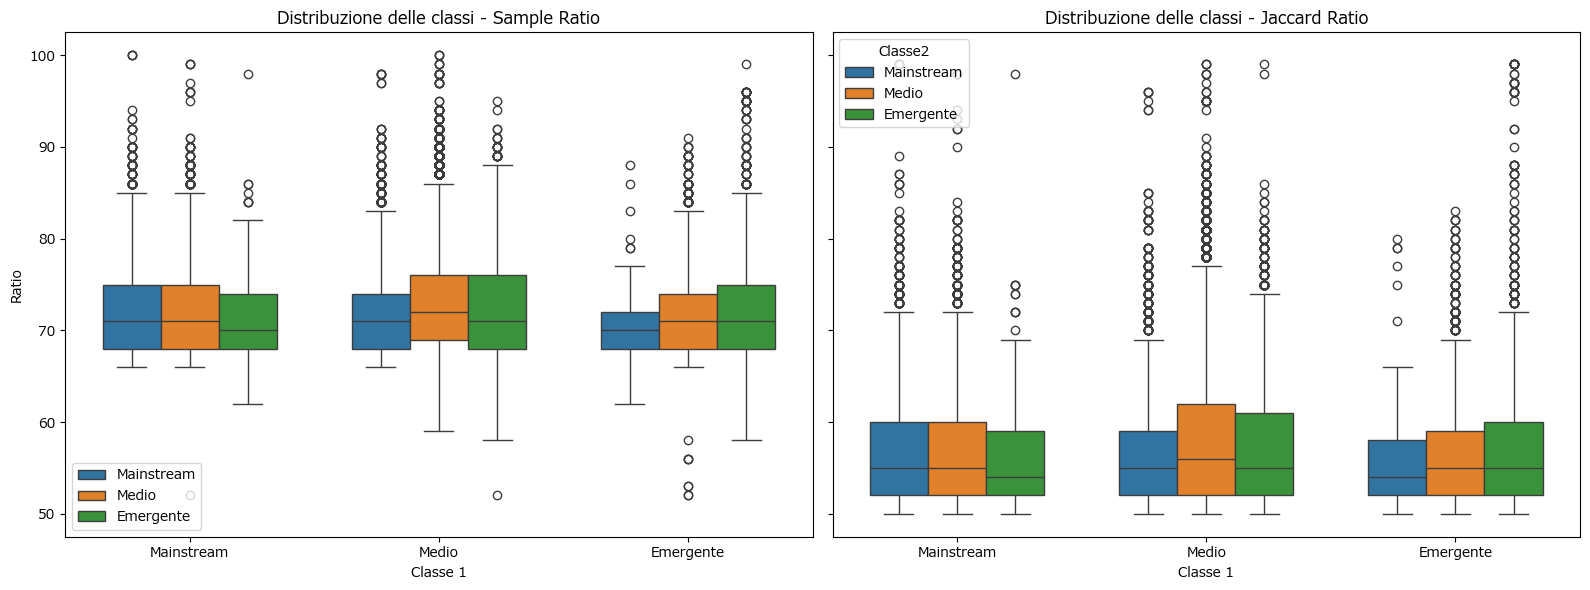
\includegraphics[width=0.45
\textwidth]{../open_problem/plots/3_2/clDist.png}
\caption{Distribuzione degli archi per Ratio e classe}
\label{fig:clDist}
\end{figure}

\noindent Sul {\itshape Sample} Ratio, il numero di artisti simili condivisi (in proporzione) è relativamente omogeneo tra le classi. Tuttavia, potrebbero esserci più outlier o interazioni più diverse quando sono coinvolti artisti emergenti. Invece, lo {\itshape Jaccard} Ratio, penalizza le coppie con ampio numero di artisti simili non condivisi. Gli artisti medi condividono una frazione maggiore del loro universo simile, mentre i mainstream hanno insiemi più grandi e meno sovrapposti. \\ \\ In seguito si è preso in considerazione un subgraph del grafo (si considera il primo) e si rappresentano le classi di riferimento.

\begin{figure}[H]
\centering
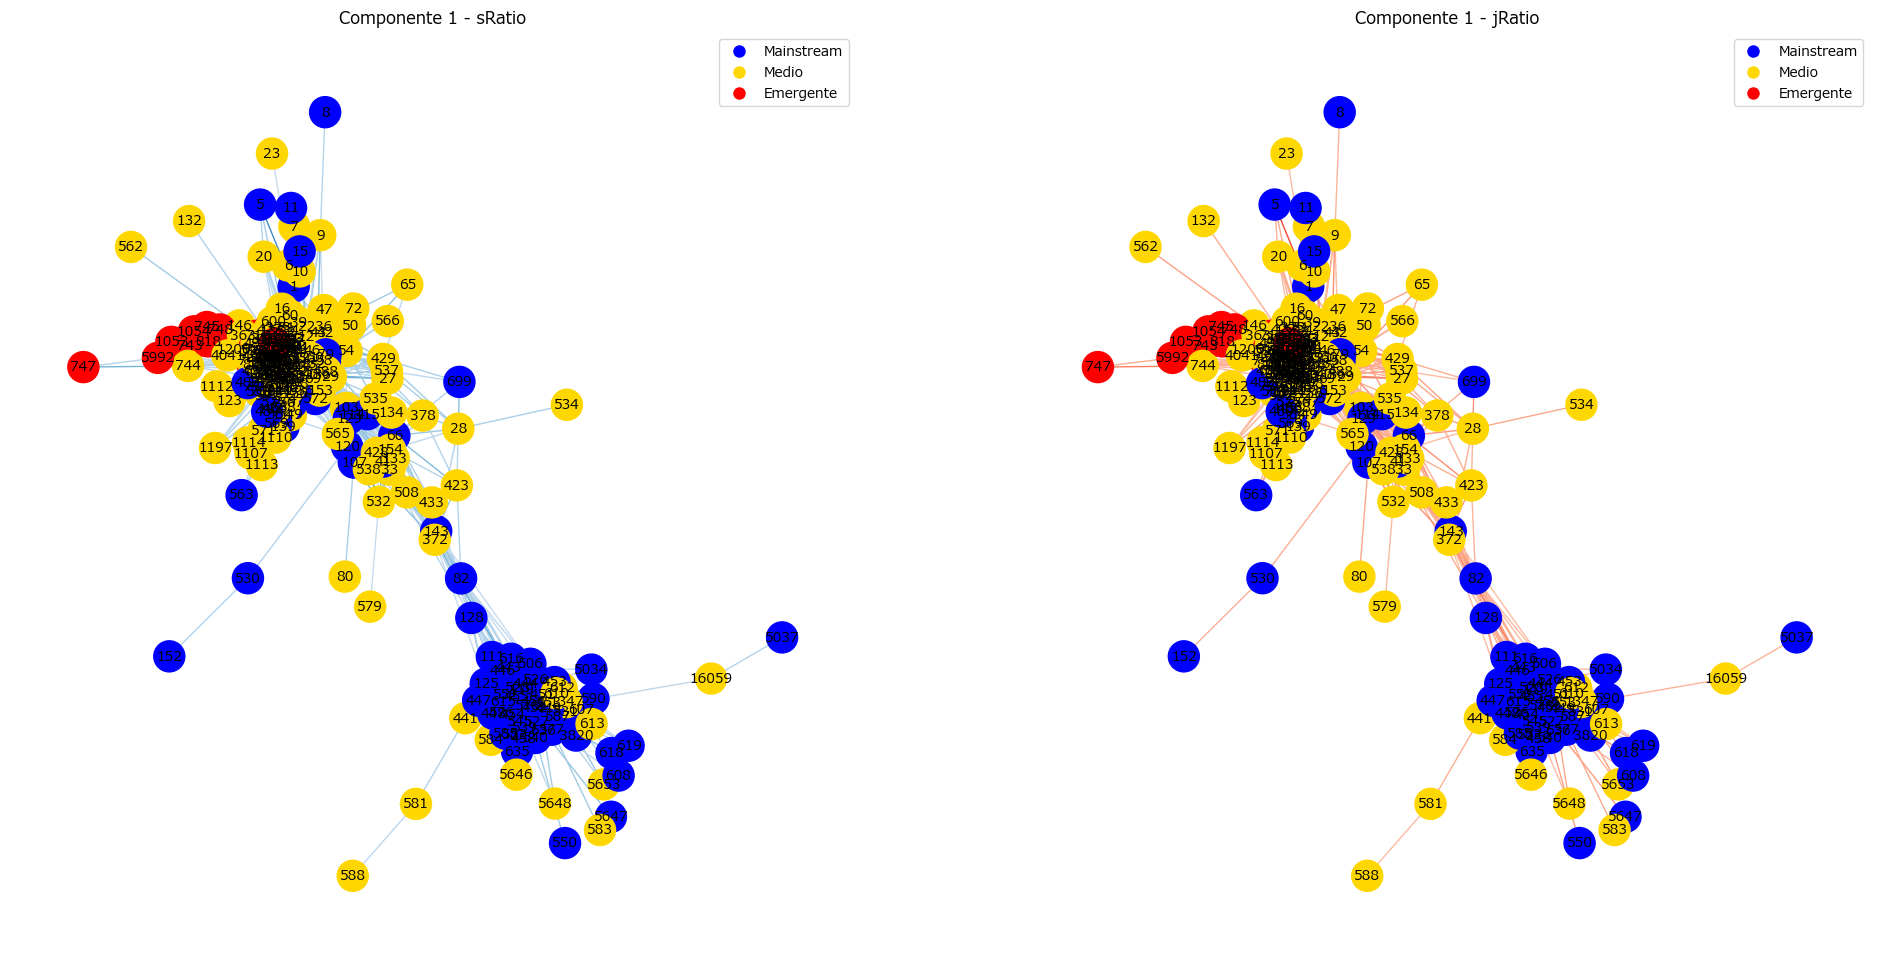
\includegraphics[width=0.45
\textwidth]{../open_problem/plots/3_2/clSubgraph_1.png}
\caption{Subgraph 1 con classificazione}
\label{fig:clSubgraph_1}
\end{figure}

\noindent Di questo sottografo è interessante notare che esiste una community composta quasi totalmente da artisti mainstream; in più ne esiste un'altra formata per la maggiore da artisti medi. Infine, gli emergenti corrispondono a una piccola parte del {\itshape subgraph}.

\subsection{Calcolo delle classi intermedie}

Stabilite le classi degli artisti, è utile in questa fase individuare quali sono gli artisti che possono tendere a un aumento o a un calo di popolarità. Per far ciò sono state analizzate le community, ricercate attraverso l'algoritmo di Louvain, in cui è presente ciascun artista. In primo luogo per ciascuna community sono stati calcolati lo Z-Index, il Sample e lo Jaccard medi. Lo studio delle community è utile per identificare il contesto e trovare cluster potenzialmente interessanti e non per cambiare direttamente la classe di un artista; la community da sola non è una buona predittrice della struttura interna o della popolarità.
 \\ \\ Quindi si definiscono altre tre classi per identificare i nodi che possono tendere ad un cambio di classe: chi potrebbe tornare a diventare di nicchia, chi potrebbe essere un possibile medio e chi potrebbe essere un possibile mainstream. Si contano i vicini di ogni nodo per classe e, per ciascuno:

\begin{itemize}
\item diventa possibile mainstream se è emergente o medio e ha almeno due vicini mainstream.
\item diventa possibile medio se è mainstream/emergente e ha almeno due vicini emergenti/mainstream.
\item può tornare emergente se è mainstream/medio e ha almeno tre vicini emergenti.
\end{itemize}
Svolti i calcoli opportuni, prendendo il primo {\itshape subgraph} si ottiene qualcosa del tipo:

\begin{figure}[H]
\centering
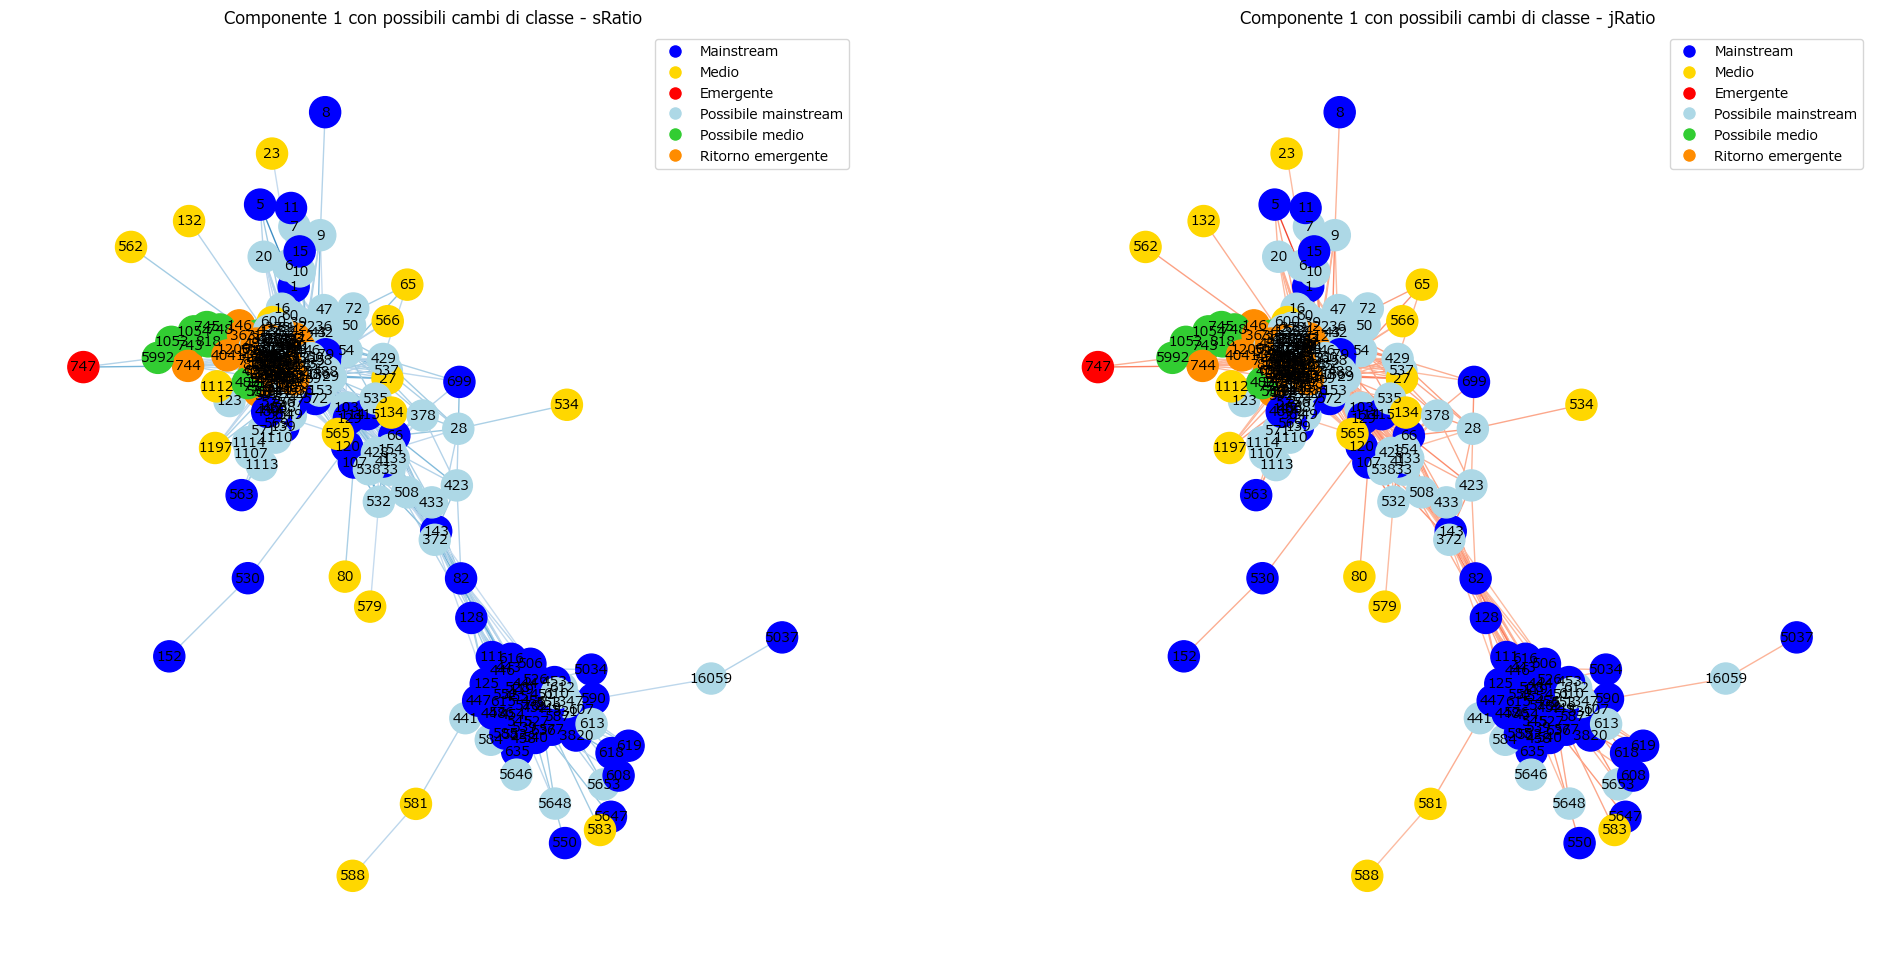
\includegraphics[width=0.45
\textwidth]{../open_problem/plots/3_3/subClSubgr_1.png}
\caption{Subgraph 1 con classificazione intermedia}
\label{fig:subClSubgr_1}
\end{figure}

\subsection{Previsione del trend}

Definite le classi principali degli artisti ({\itshape mainstream}, {\itshape medio} ed {\itshape emergente}) e quelle intermedie ({\itshape possibile mainstream}, {\itshape possibile medio}, {\itshape ritorno emergente}) si prova a prevedere il {\itshape trend}, ovvero se c'è una possibilità di crescita, di calo o se la popolarità di quell'artista resti stabile. Per far ciò sono stati adoperati dei coefficienti di correlazione per ciascun artista:

\begin{itemize}
\item la {\itshape Degree Centrality}, poiché se un artista ha un grado alto ha più possibilità di farsi conoscere e quindi ottenere maggiore popolarità;
\item il coefficiente di {\itshape clustering}, perché può considerarsi stabile e quindi più "protetto" da altri colleghi con popolarità maggiore;
\item la {\itshape Betweenness Centrality}, in quanto ha la possibilità di diventare un {\itshape trend setter} o, se già conosciuto, consolidare maggiormente la sua popolarità;
\item il {\itshape PageRank}, perché misura l'importanza dell'artista in base non solo al numero di collegamenti, ma anche all'importanza di chi lo collega, quindi può misurare un potenziale {\itshape glow-up}.
\end{itemize}

I coefficienti di correlazione ricavati dai calcoli sono dunque i seguenti:

\begin{table}[H]
\centering
\small
\begin{tabular}{l r}
\hline
\textbf{Degree} & 0.002 \\
\textbf{Clustering} & -0.038 \\
\textbf{Betweenness} & 0.010 \\
\textbf{PageRank} & 0.043 \\
\textbf{Sample medio} & 0.005 \\
\textbf{Jaccard medio} & -0.012 \\
\hline
\end{tabular}
\caption{Coefficiente di correlazione tra metriche strutturali e Z-Index della popolarità}
\label{tab:corrMetrics}
\end{table}
A questi parametri si aggiungono anche il Sample e lo Jaccard Ratio medi, cioè rispettivamente quanto un artista è simile mediamente ai suoi collegamenti e quanto il set di artisti simili è sovrapposto. \\ \\ Per ogni artista viene quindi creato un vettore con tali parametri, dunque si dà vita a una {\bfseries matrice di correlazione} tra questi e lo Z-Index. I criteri, dunque, per distinguere un trend di crescita da uno in calo si possono riassumere in questo modo.
Si considera un artista in {\bfseries trend positivo} se:

\begin{itemize}
	\item è {\itshape emergente} o {\itshape medio} e:
	\begin{itemize}
		\item il PageRank è superiore al $70^\circ$ percentile;
		\item il Sample Ratio medio è superiore a $85$ e lo Jaccard medio a $75$;
	\end{itemize}
	\item la Betweenness è superiore al $75^\circ$ percentile se di rango medio.
\end{itemize}
Al contrario, un artista è in {\bfseries trend negativo} se:

\begin{itemize}
\item è {\itshape emergente} o {\itshape medio};
\item il PageRank è superiore al $70^\circ$ percentile
\item il Sample Ratio medio è superiore a $85$ e lo Jaccard medio a $75$;
\item la Betweenness è superiore al $75^\circ$ percentile se di rango medio.
\end{itemize}

\noindent Dunque è stata creata una {\itshape heat map} con gli artisti, di ciascuna classe, che possono avere un trend positivo o negativo, o che rimane stabile:

\begin{figure}[H]
\centering
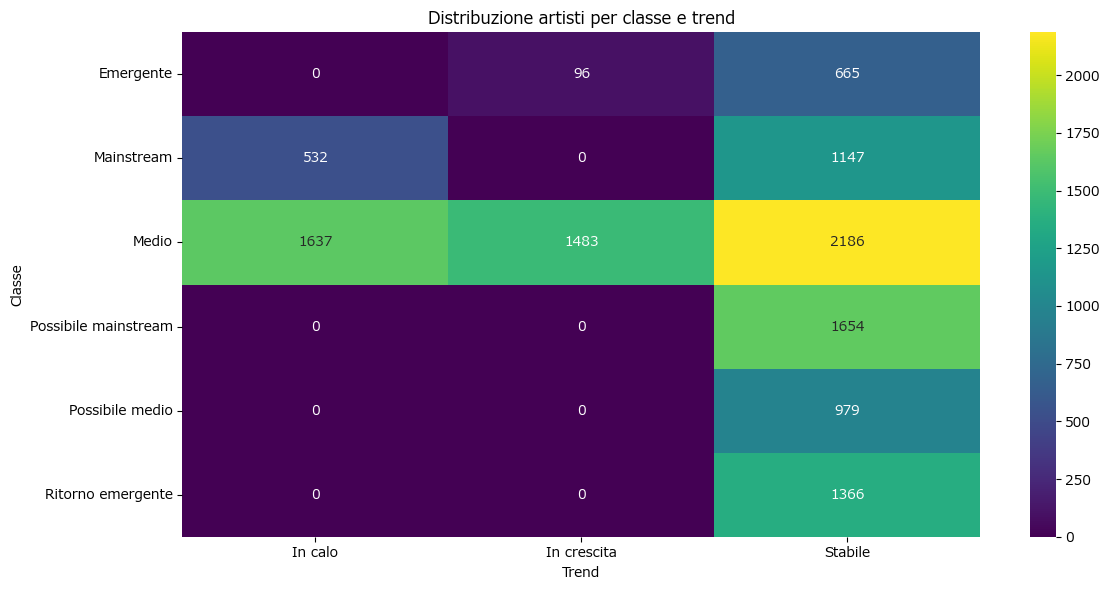
\includegraphics[width=0.45
\textwidth]{../open_problem/plots/3_4/clTrendDist.png}
\caption{Distribuzione artisti per classe e trend}
\label{fig:clTrendDist}
\end{figure}

\noindent Dall'analisi della distribuzione degli artisti per classe e trend emergono alcune dinamiche interessanti. Gli artisti \textit{medi} sono più dinamici, con una significativa presenza sia di casi in crescita sia in calo, il che fa intendere che, data la posizione "centrale" della gerarchia, si tratta di un comportamento plausibile. Gli \textit{emergenti}, invece, sono per la maggiore stabili, ma una parte mostra segnali di crescita, indicando possibilità di affermazione futura. Infine, tra i \textit{mainstream}, oltre alla stabilità, si osserva una quota rilevante di artisti in calo, suggerendo che mantenere una posizione di vertice può risultare complesso. Le classi intermedie, infine, si mantengono invece stabili, come da definizione. \\ \\ Complessivamente i medi si confermano i più esposti a cambiamenti, mentre le altre categorie mostrano maggiore inerzia. \\ \\ Per concludere si sono ricavati artisti emergenti possono fare un glow up (ovvero quelli promettenti), mostrando le community in cui sono presenti e, al contrario, i mainstream che possono invece perdere popolarità. \\ \\ Sono stati selezionati, infine, alcuni artisti emergenti con potenziale crescita e artisti mainstream in calo, sulla base dei loro indici strutturali e di popolarità. Per ciascun artista è stata individuata la community di appartenenza e rappresentata graficamente la rete locale, con l'obiettivo di analizzare come la posizione nella rete possa favorire un cambiamento di trend. Come esempio sono stati analizzati gli Snap! come possibile {\itshape glow up} e Shakira come possibile {\itshape glow down}:

\begin{figure}[H]
\centering

\begin{subfigure}{0.45\textwidth}
  \centering
  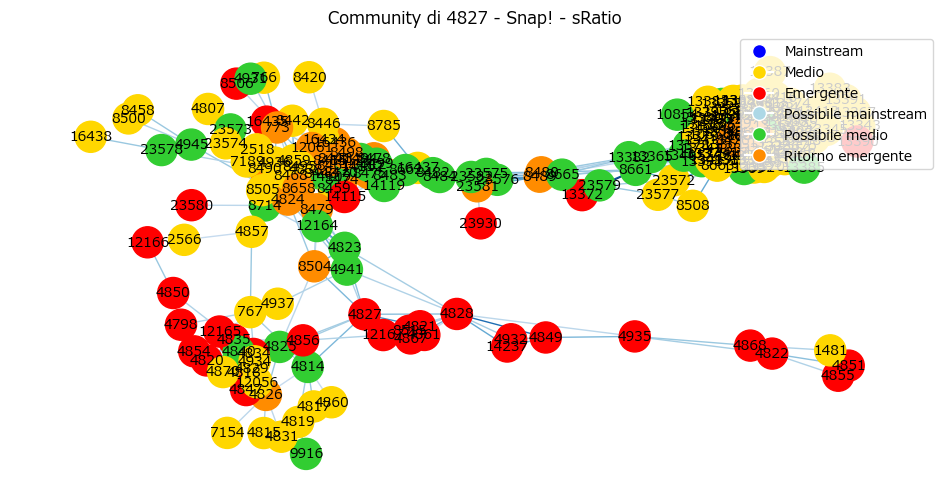
\includegraphics[width=\linewidth]{../open_problem/plots/3_4/comm4827_sRatio.png}
  \caption{Community degli Snap! - Crescente}
\end{subfigure}
\hfill
\begin{subfigure}{0.45\textwidth}
  \centering
  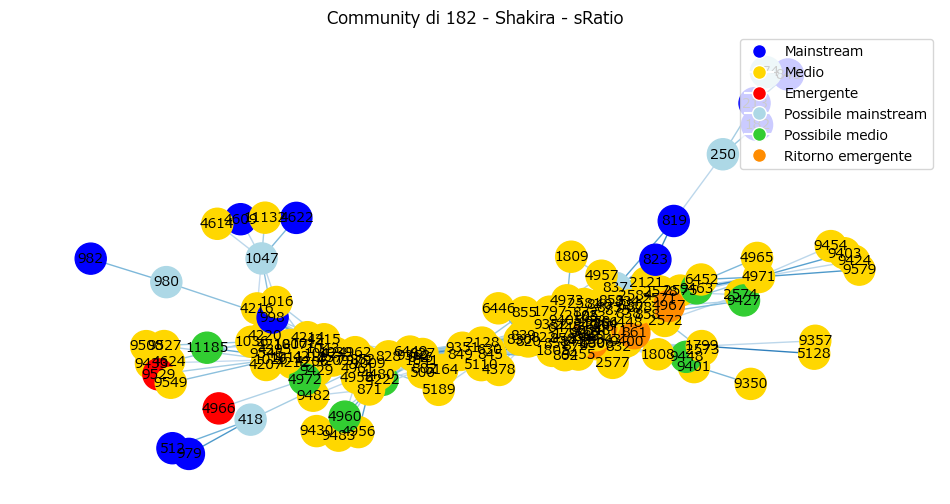
\includegraphics[width=\linewidth]{../open_problem/plots/3_4/comm182_sRatio.png}
  \caption{Community di Shakira - In calo}
\end{subfigure}

\caption{Esempi di community di artisti con trend positivo/negativo}
\label{fig:trendComm}
\end{figure}


\section{Discussion}
Il progetto ha mostrato come l'analisi delle relazioni di similarità tra artisti musicali possa offrire spunti interessanti per comprendere le dinamiche di crescita o declino nella popolarità. Attraverso metriche strutturali e coefficienti di similarità, è stato possibile individuare tendenze e potenziali cambi di status tra artisti emergenti, medi e mainstream. \\ \\ L'integrazione di dati strutturali e di popolarità ha permesso non solo di descrivere la rete, ma anche di fornire modelli predittivi semplici e interpretabili. Sebbene i risultati siano incoraggianti, ulteriori sviluppi potrebbero prevedere l'integrazione di dati temporali o l'uso di modelli predittivi più complessi per affinare l'analisi.

% The next two lines define the bibliography style to be used, and the bibliography file.
\bibliographystyle{ACM-Reference-Format}
\bibliography{biblio}

\end{document}

